\chapter{Fundamentação Técnica e Arquitetura do Sistema}

Esta seção apresenta a arquitetura da interface musical multissensorial e os fundamentos técnicos necessários para compreender seu funcionamento. A solução foi organizada em módulos de entrada, processamento computacional, comunicação, controle embarcado, alimentação e saída sensorial. Essa separação permite analisar individualmente as etapas da cadeia e facilita modificações posteriores sem exigir a substituição integral da plataforma.

A informação utilizada pelo sistema é obtida diretamente durante a interação com o controlador MIDI. O parâmetro \textit{velocity} é processado no computador, convertido em um comando PWM e transmitido ao ESP32 por UDP sobre rede Wi-Fi. O microcontrolador utiliza esse comando como referência para o motor vibrotátil e para o LED da unidade vestível.

\section{Visão Geral da Arquitetura}
\markright{Fundamentação Técnica e Arquitetura do Sistema}
\label{sec:visao_geral_arquitetura}

A arquitetura relaciona a intensidade do gesto realizado sobre os \textit{pads} do Akai MPD218 a duas respostas físicas. O controlador permanece conectado ao computador por USB e envia as mensagens MIDI geradas durante a execução. O software em Python interpreta esses eventos, calcula o nível de controle e transmite o comando ao ESP32 por uma rede Wi-Fi.

A unidade embarcada recebe os datagramas UDP e atualiza duas saídas independentes: o GPIO 18 controla o estágio eletrônico do motor Vibracall 1027 e o GPIO 21 controla o LED de alto brilho. Embora as saídas sejam distintas, ambas utilizam o mesmo valor digital como referência.

A alimentação da unidade vestível é local. Duas células 18650 em configuração 2S são associadas a um módulo BMS e a um conversor DC--DC ajustado para aproximadamente 3,3~V. Essa configuração elimina cabos entre o computador e o módulo vestível durante a operação normal, mas não torna todo o sistema sem fio, pois o controlador MIDI continua conectado ao computador por USB.

A Figura~\ref{fig:fluxograma_sistema} apresenta os principais blocos da arquitetura e o fluxo de informação entre eles.

\begin{figure}[!htbp]
\centering
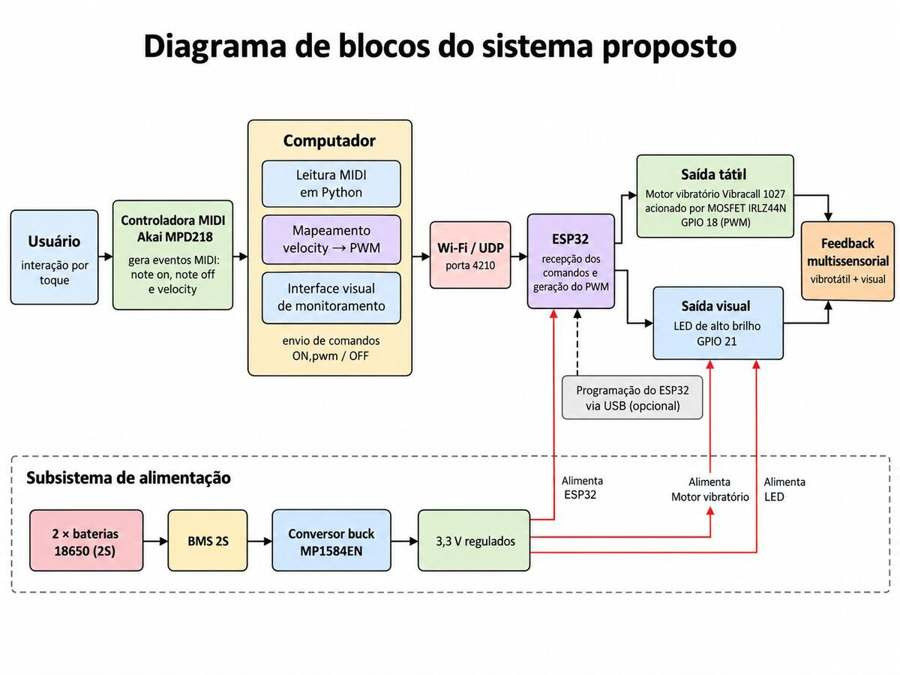
\includegraphics[
width=0.96\linewidth,
keepaspectratio
]{Imagens/Diagramas/diagrama_blocos_sistema.jpg}
\caption{Diagrama de blocos da arquitetura funcional do sistema desenvolvido}
\label{fig:fluxograma_sistema}
\legend{Fonte: Elaboração própria (2026).}
\end{figure}

\section{Interface Musical Digital e Protocolo MIDI}
\markright{Fundamentação Técnica e Arquitetura do Sistema}
\label{sec:interface_midi}

A interface de entrada é baseada no controlador Akai MPD218. O dispositivo converte o acionamento de seus \textit{pads} em mensagens MIDI, disponibilizadas ao computador por USB \cite{akai2015mpd218}.

O protocolo MIDI não transporta o sinal de áudio do instrumento. As mensagens representam eventos da execução, como acionamento e liberação de notas, identificação do elemento acionado e parâmetros de dinâmica \cite{midi1996}. Essa característica permite utilizar informações do gesto antes da geração do som, o que é adequado à proposta de comandar modalidades sensoriais paralelas à saída musical.

\subsection{Controlador MIDI Akai MPD218}
\label{subsec:mpd218}

O MPD218 possui 16 \textit{pads} utilizados como superfície principal de interação. O controlador envia ao computador mensagens que incluem a nota MIDI e o valor de \textit{velocity} associado ao acionamento \cite{akai2015mpd218}. No protótipo, a nota identifica visualmente o \textit{pad} correspondente, enquanto a \textit{velocity} é utilizada no cálculo do nível de controle.

A Figura~\ref{fig:mpd218_esquematico} apresenta uma representação esquemática da disposição dos controles do MPD218.



O controlador não seleciona diferentes motores no sistema desenvolvido. A configuração final utiliza um único atuador vibrotátil, de modo que a identificação da nota permanece vinculada à interface gráfica e ao registro dos eventos.

\begin{figure}[!htbp]
\centering
\resizebox{0.93\linewidth}{!}{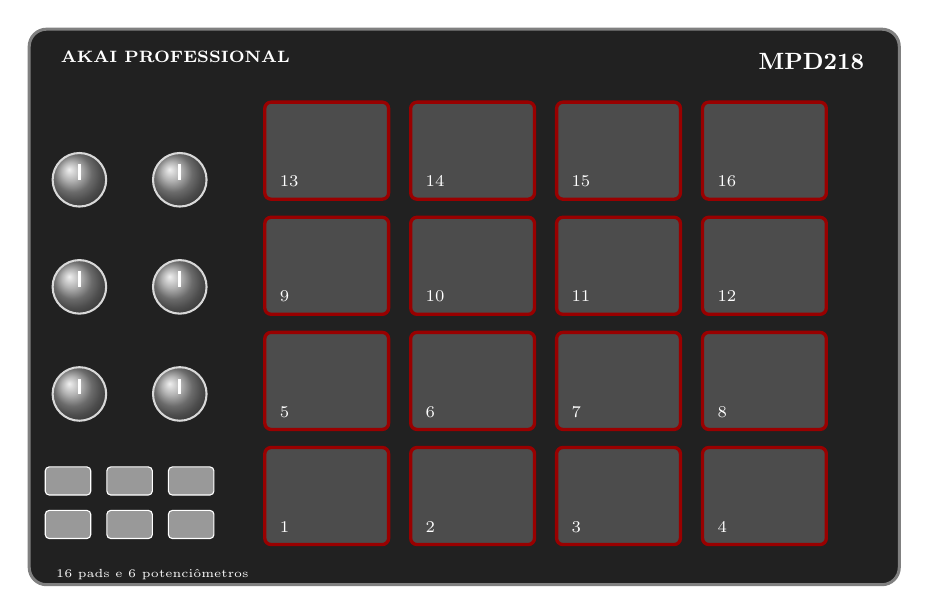
\begin{tikzpicture}[x=1cm,y=1cm,scale=0.85,every node/.style={transform shape}]
\draw[rounded corners=0.22cm,fill=black!87,draw=black!50,line width=1.1pt] (0,0) rectangle (13,8.3);
\node[anchor=west,text=white,font=\bfseries\scriptsize] at (0.35,7.88) {AKAI PROFESSIONAL};
\node[anchor=east,text=white,font=\bfseries] at (12.6,7.82) {MPD218};
\foreach \y in {2.85,4.45,6.05}{
 \foreach \x in {0.75,2.25}{
  \shade[ball color=black!40] (\x,\y) circle (0.39);
  \draw[draw=black!15,line width=0.75pt] (\x,\y) circle (0.40);
  \draw[draw=white!70,line width=1pt] (\x,\y) -- ++(0,0.23);
 }
}
\foreach \i in {0,1,2,3}{
 \foreach \j in {0,1,2,3}{
  \pgfmathtruncatemacro{\padnum}{4*\i+\j+1}
  \draw[fill=black!70,draw=red!60!black,line width=1.2pt,rounded corners=0.08cm]
    (3.52+2.18*\j,0.60+1.72*\i) rectangle (5.37+2.18*\j,2.05+1.72*\i);
  \node[anchor=south west,text=white,font=\scriptsize] at (3.62+2.18*\j,0.66+1.72*\i) {\padnum};
 }
}
\foreach \y in {0.90,1.55}{
 \foreach \x in {0.58,1.50,2.42}{
  \draw[fill=black!40,draw=white!50,rounded corners=0.05cm]
    (\x-0.34,\y-0.21) rectangle (\x+0.34,\y+0.21);
 }
}
\node[text=white,font=\tiny,align=left,anchor=west] at (0.28,0.15) {16 pads e 6 potenciômetros};
\end{tikzpicture}
}
\caption{Representação esquemática do controlador Akai MPD218, com 16 \textit{pads} e seis potenciômetros}
\label{fig:mpd218_esquematico}
\legend{Fonte: Elaboração própria, com base em \textcite{akai2015mpd218}.}
\end{figure}

\subsection{Mensagens MIDI e Parâmetro \textit{Velocity}}
\label{subsec:velocity_midi}

Entre as mensagens relevantes para a aplicação estão \textit{note\_on} e \textit{note\_off}. No MIDI 1.0, o campo \textit{velocity} é codificado em sete bits e admite valores de 0 a 127. Um evento \textit{note\_on} com \textit{velocity} igual a zero também pode representar o encerramento da nota \cite{midi1996}.

A \textit{velocity} fornece uma variável digital associada à dinâmica do acionamento. Neste trabalho, seu valor é empregado como entrada para uma função de mapeamento implementada em Python. A saída dessa função é o valor PWM transmitido ao ESP32.

A relação funcional pode ser representada por

\begin{equation}
V_{\mathrm{MIDI}}
\longrightarrow
f(V_{\mathrm{MIDI}})
\longrightarrow
P_{\mathrm{PWM}}
\longrightarrow
\left\{
\begin{array}{l}
\text{feedback vibrotátil}\\
\text{feedback visual}
\end{array}
\right.,
\end{equation}

em que $V_{\mathrm{MIDI}}$ representa a \textit{velocity}, $f(\cdot)$ corresponde ao mapeamento implementado no software e $P_{\mathrm{PWM}}$ é o comando utilizado pelas saídas.

A escolha dessa variável não implica equivalência entre gesto e intensidade percebida. O mapeamento estabelece uma relação de controle; a resposta mecânica do motor, a resposta luminosa do LED e a percepção humana possuem características próprias e são tratadas separadamente nas limitações do trabalho.

\section{Arquitetura do Sistema Proposto}
\markright{Fundamentação Técnica e Arquitetura do Sistema}
\label{sec:arquitetura_sistema}

O sistema pode ser dividido em seis módulos funcionais. A interface musical registra o gesto do usuário; o processamento computacional interpreta as mensagens MIDI e calcula o comando; a comunicação transfere esse comando ao módulo embarcado; o ESP32 gera as saídas; o sistema de alimentação fornece energia localmente; e os elementos de \textit{feedback} convertem o comando em respostas tátil e visual.

Essa organização modular permite alterar individualmente a interface de entrada, a função de mapeamento, o protocolo de comunicação, o atuador ou a forma de alimentação. No protótipo validado, os módulos foram integrados em uma cadeia única, mas permaneceram testáveis de forma independente.

O protocolo UDP opera por datagramas e não fornece, por si só, mecanismos de confirmação de entrega, ordenação ou retransmissão \cite{postel1980udp}. Sua utilização foi escolhida pela simplicidade da troca de mensagens curtas e pela baixa sobrecarga para a aplicação em rede local. A confiabilidade observada no ensaio realizado é discutida no Capítulo 5 e não é generalizada para outras condições de rede.

\section{Unidade de Controle Embarcada}
\markright{Fundamentação Técnica e Arquitetura do Sistema}
\label{sec:esp32}

A unidade de controle embarcada utiliza um módulo ESP32-WROOM-32 instalado em uma placa de desenvolvimento com conector micro-USB. O ESP32 concentra a recepção dos comandos e a geração das saídas do módulo vestível. O dispositivo possui conectividade Wi-Fi integrada e periféricos destinados à geração de sinais PWM, características compatíveis com a arquitetura proposta \cite{espressif2026esp32,espressifledc}.

O processamento musical permanece no computador. O microcontrolador recebe comandos já convertidos para a faixa de controle e não interpreta diretamente o protocolo MIDI. Essa divisão reduz a complexidade do software embarcado e separa o tratamento dos eventos musicais da atuação física.

Após a recepção de um comando válido, o ESP32 atualiza o canal do motor e o canal do LED. O motor não é alimentado diretamente pelo GPIO; o pino controla o MOSFET, enquanto a corrente do atuador é fornecida pelo barramento regulado. O LED, por sua vez, é acionado por uma saída dedicada com resistor limitador de corrente.

\section{Sistema de Feedback Multissensorial}
\markright{Fundamentação Técnica e Arquitetura do Sistema}
\label{sec:feedback_vibrotatil}

As saídas do sistema foram definidas para apresentar a mesma informação de controle por duas modalidades. O motor Vibracall 1027 produz o \textit{feedback} vibrotátil e o LED de alto brilho produz o \textit{feedback} visual.

O mesmo valor PWM é utilizado como referência para as duas saídas, mas essa decisão não estabelece equivalência perceptiva entre elas. Um valor digital comum pode produzir respostas físicas com relações distintas de amplitude, frequência, brilho e percepção. O compartilhamento do comando deve ser entendido apenas como sincronização funcional das modalidades.

A proposta também não reproduz o conteúdo acústico do MIDI. Nota, timbre e frequência sonora não são convertidos diretamente em frequência de vibração ou cor. O sistema representa eventos da interação e sua intensidade relativa, preservando o instante de acionamento e o valor de controle calculado.

\section{Fluxo de Funcionamento Durante a Interação}
\markright{Fundamentação Técnica e Arquitetura do Sistema}
\label{sec:fluxo_funcionamento}

Cada acionamento de um \textit{pad} gera uma mensagem MIDI recebida pelo programa. Para eventos válidos, a nota é utilizada na identificação visual e a \textit{velocity} é convertida para o valor PWM correspondente. O comando é transmitido por UDP ao ESP32, que atualiza o GPIO 18 e o GPIO 21. Dessa forma, o evento produz respostas vibrotátil e visual sincronizadas ao mesmo comando digital.

Quando a liberação do \textit{pad} é identificada, o software transmite \texttt{OFF}, interrompendo as duas saídas. O fluxo funcional pode ser sintetizado por

\begin{equation}
\begin{split}
\text{Gesto}
&\rightarrow
\text{Evento MIDI}
\rightarrow
\textit{Velocity}\\
&\rightarrow
\text{Processamento em Python}
\rightarrow
\text{UDP/Wi-Fi}\\
&\rightarrow
\text{ESP32}
\rightarrow
\text{PWM}
\rightarrow
\begin{cases}
\text{feedback vibrotátil}\\
\text{feedback visual}.
\end{cases}
\end{split}
\end{equation}

A interface gráfica é atualizada em paralelo à transmissão. A unidade vestível permanece alimentada localmente, sem cabo de dados ou alimentação para o computador.
